\documentclass{beamer}

% Prévoir à peu près un transparent par minute d'exposé.
% Deux ou trois sections semble être une bonne chose.

\mode<presentation>
{
  \usetheme{Darmstadt}
  % ou ...

  \setbeamercovered{transparent}
  % ou autre chose (ou on l'enlève)
}

\usecolortheme{seahorse}

\usepackage[french]{babel}
\usepackage[utf8]{inputenc}
\usepackage{times}
\usepackage{verbatim}
\usepackage[T1]{fontenc}
\usepackage{listings}
\RequirePackage[lined,boxed,commentsnumbered]{algorithm2e}

\title[NuQleosim]
{
  NuQleosim
}

\subtitle
{}

\author[Laetitia Bourgeade Hadrien Mary Florence Maurier Jean-Paul Navailles]
{Laetitia Bourgeade \\ Hadrien Mary \\ Florence Maurier \\ Jean-Paul Navailles}

\institute[Universités Bordeaux 1 \& 2]
{
  Universités Bordeaux 1 \& 2
}

%% Insertion du logo
% \begin{columns}
%   \begin{right}
%     
\includegraphics[width=0.3\columnwidth]{logo/uni.png}
%   \end{right}
% \end{columns}

\date{Février 2011} % (optionnel, abbréviation du nom de la conférence)

% Effacer cela si vous ne voulez pas que la table des matières
% apparaisse au début de chaque section
\AtBeginSection[]
{
  \begin{frame}<beamer>
    \frametitle{Rappel du plan}
    \tableofcontents[currentsection]
  \end{frame}
}

\setbeamertemplate{itemize item}[ball]

\setbeamertemplate{footline}[page number]
\setbeamertemplate{navigation symbols}{}

\begin{document}

\begin{frame}
  \titlepage
\end{frame}

\section*{Introduction}

\begin{frame}
  \frametitle{Introduction}

  \begin{block}{Le nucléole}
    \begin{itemize}
    \item Localisation nucléaire 
    \item Encore mal connu
    \item Responsable de certaines pathologies
    \item Peu d'outils pour l'étude \textit{in silico}
    \end{itemize}
  \end{block}

  \begin{block}{NuQleoSim}
    \begin{itemize}
    \item Interface graphique pour l'étude du nucléole
    \item Base de donnée : moléculaire et expérimentale
    \item Modélisation de l'activité nucléolaire
    \item Gestion des résultats
    \end{itemize}
  \end{block}

\end{frame}

\begin{frame}
  \frametitle{Plan}
  \tableofcontents
\end{frame}

\section{Analyse}

\subsection{Structure et fonction}

\begin{frame}
  \frametitle{Structure}
  
  \begin{block}{}

    \begin{center}
      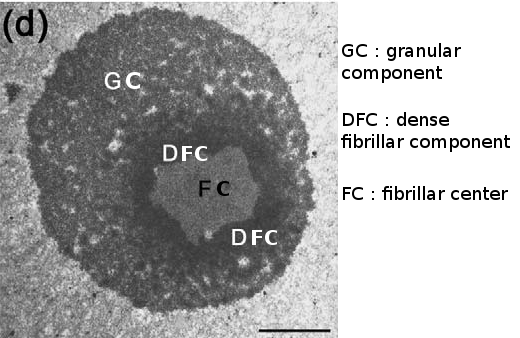
\includegraphics[width=0.6\textwidth]{img/microNuc.png}
    \end{center}

    
    Ivan Raska, Peter J Shaw, and Dusan Cmarko. \textit{Structure and function of the nucleolus in the spotlight.} Curr Opin Cell Biol, Jun 2006.
  \end{block}

\end{frame}

\begin{frame}
  \frametitle{Fonction}
  
  \begin{block}{Biogénèse des ribosomes}
  \begin{center}
    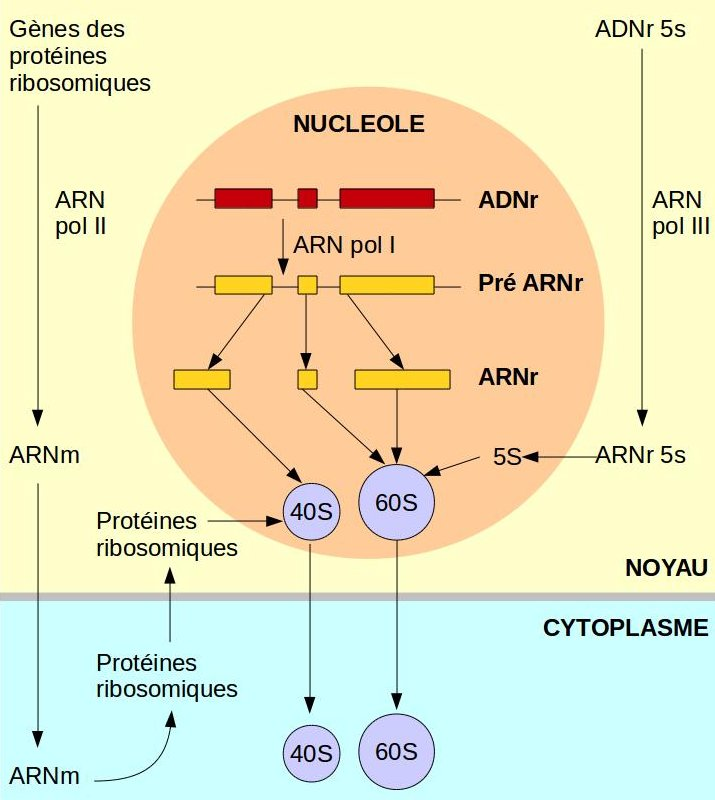
\includegraphics[width=0.5\textwidth]{img/biogenese.png}
  \end{center}
  \end{block}

\end{frame}

\subsection{Les besoins}

\begin{frame}
  \frametitle{Stockage de données}

  \begin{block}{}
    \begin{itemize}
    \item Deux types de données : moléculaire et expérimentale
    \item Création, consultation, modification et suppression
    \item Interopérabilité avec différents formats biologiques
    \end{itemize}
  \end{block}

\end{frame}

\begin{frame}
  \frametitle{Modélisation de l'activité nucléolaire}

  \begin{block}{}
    \begin{itemize}
    \item Interface de paramétrage de la simulation
    \item Communication avec la base de données
    \item Visualisation 3D en temps réel
    \item Génération de résultats
    \end{itemize}
  \end{block}

\end{frame}

\section{Conception}

\subsection{Base de données}

\begin{frame}
  \frametitle{Organisation de la base de donnée}

  \begin{block}{}
  \begin{center}
    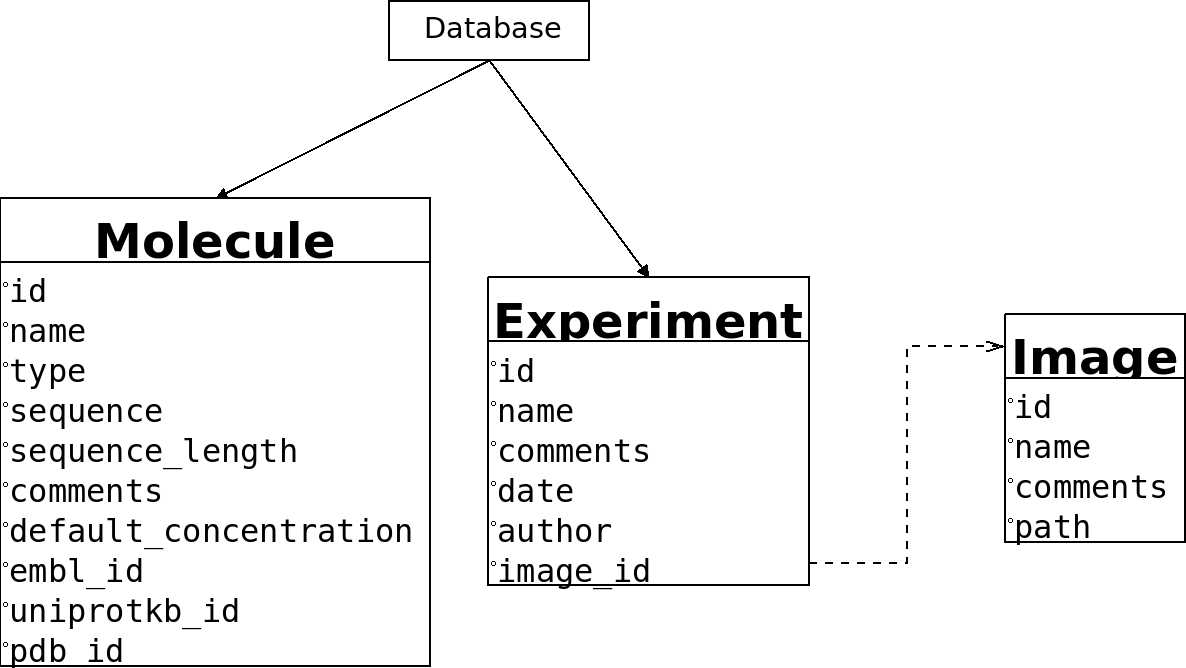
\includegraphics[width=0.4\columnwidth]{img/diagDB.png}
  \end{center}
  \end{block}

\end{frame}

\subsection{Modélisation du nucléole}

\begin{frame}
  \frametitle{Longueur et poids des protéines}

  \begin{block}{}
  \begin{center}
    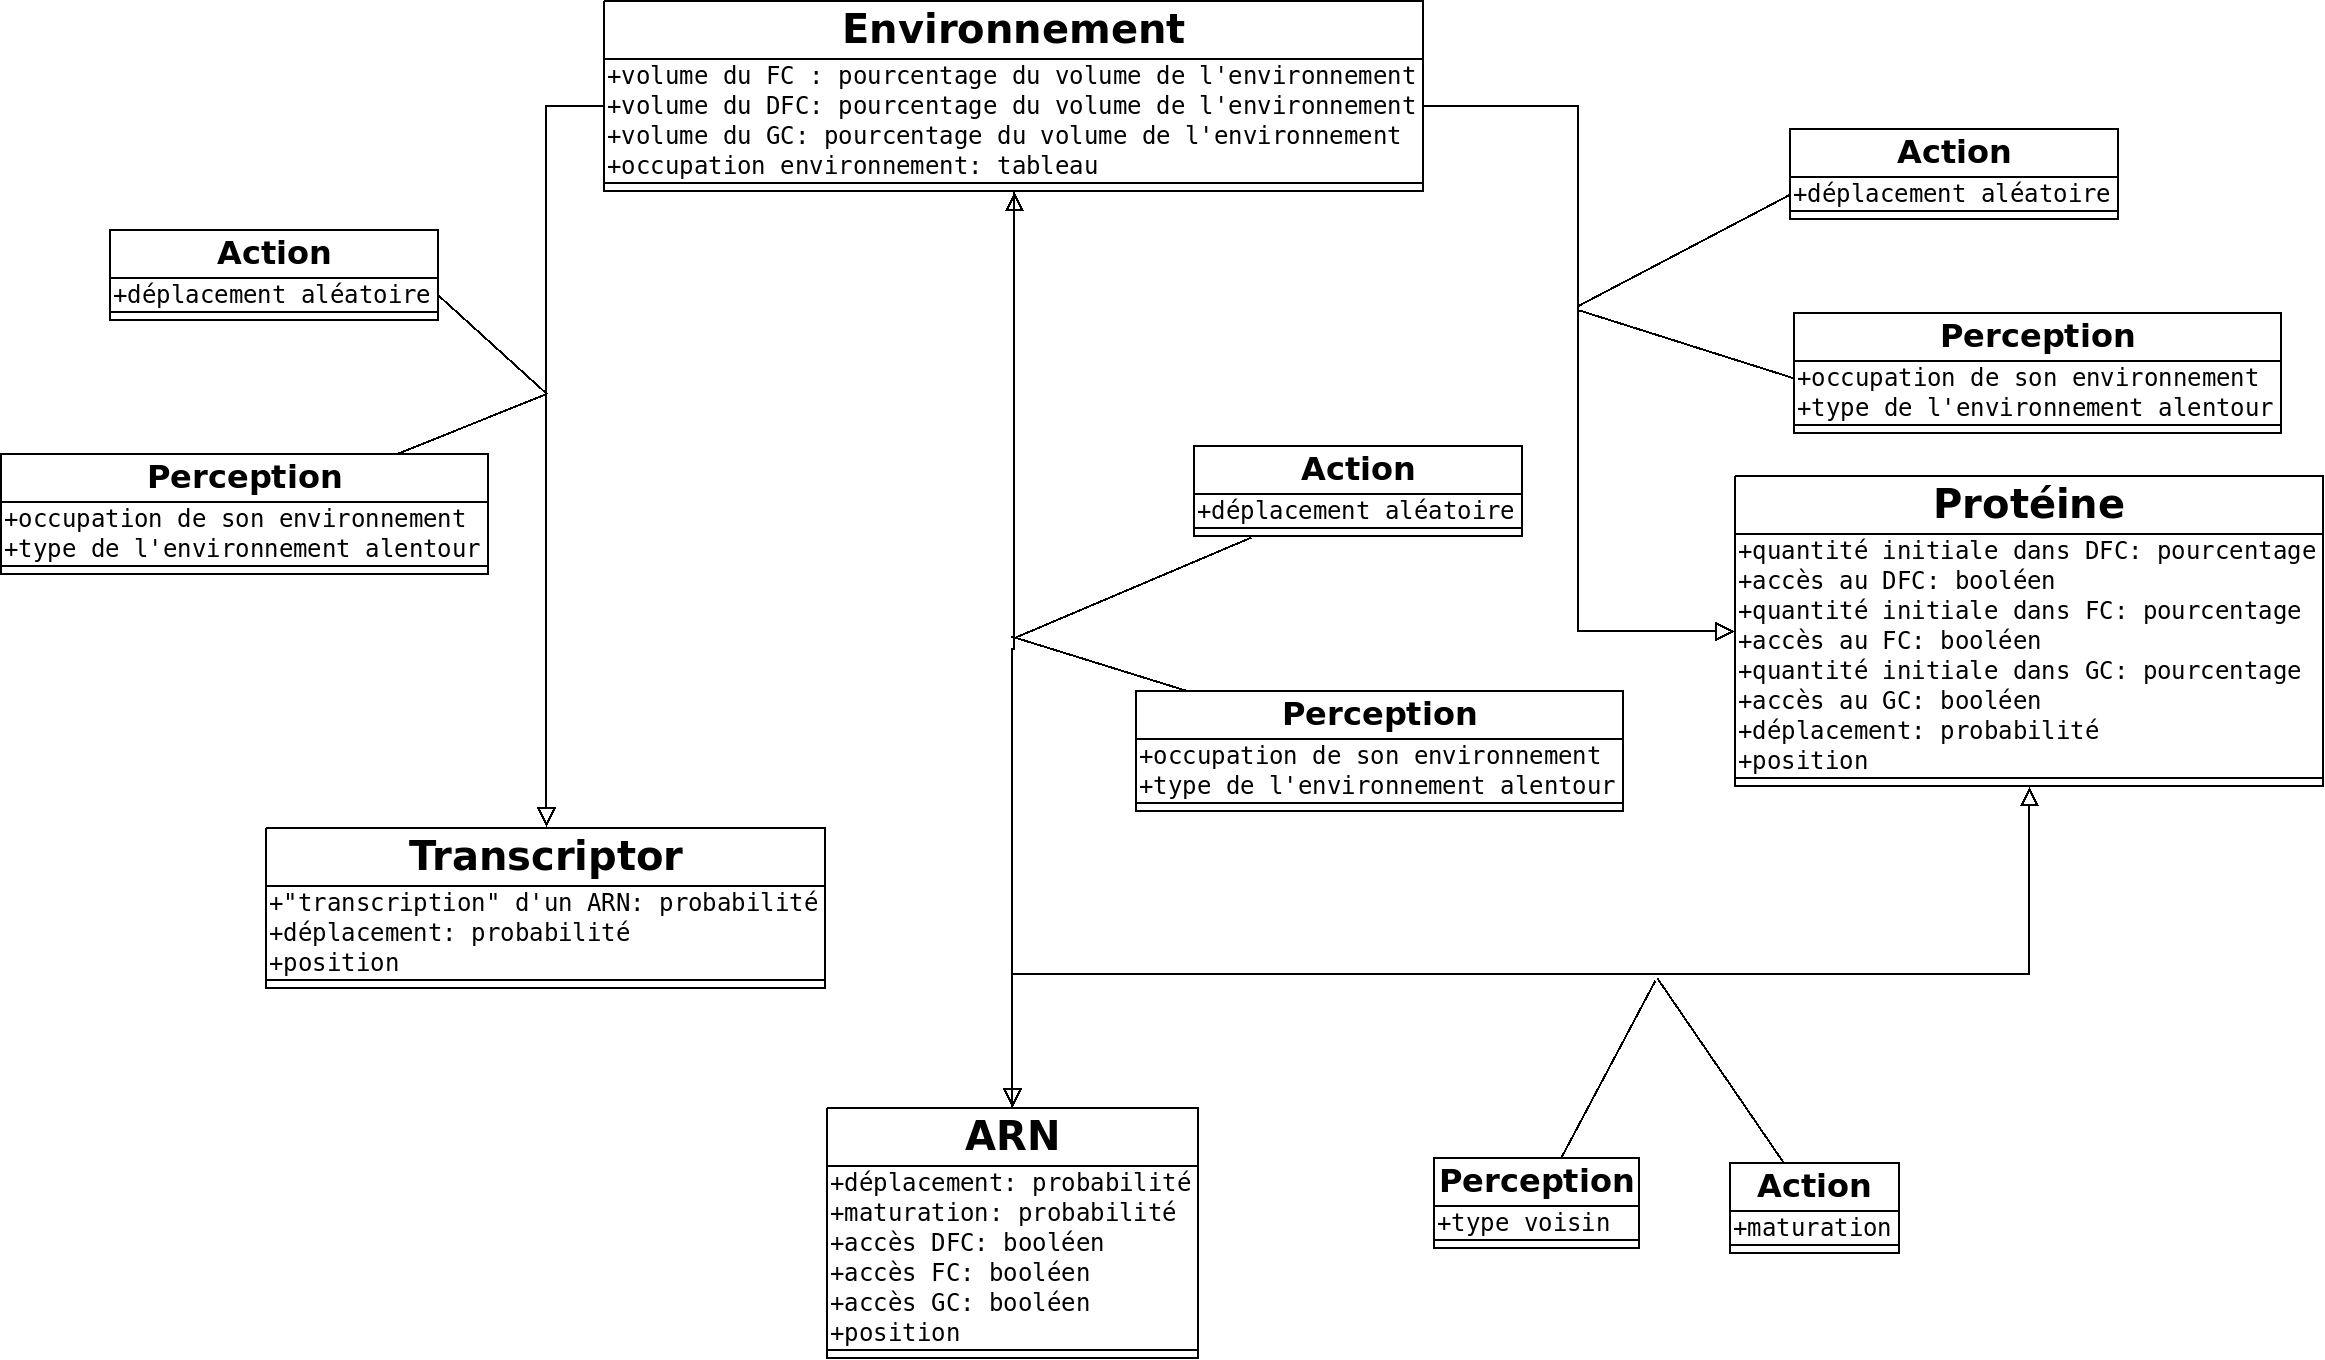
\includegraphics[width=1\columnwidth]{img/diagSMA.png}
  \end{center}
  \end{block}

\end{frame}

\begin{frame}
  \frametitle{Organisation de la base de donnée}

  \begin{center}
    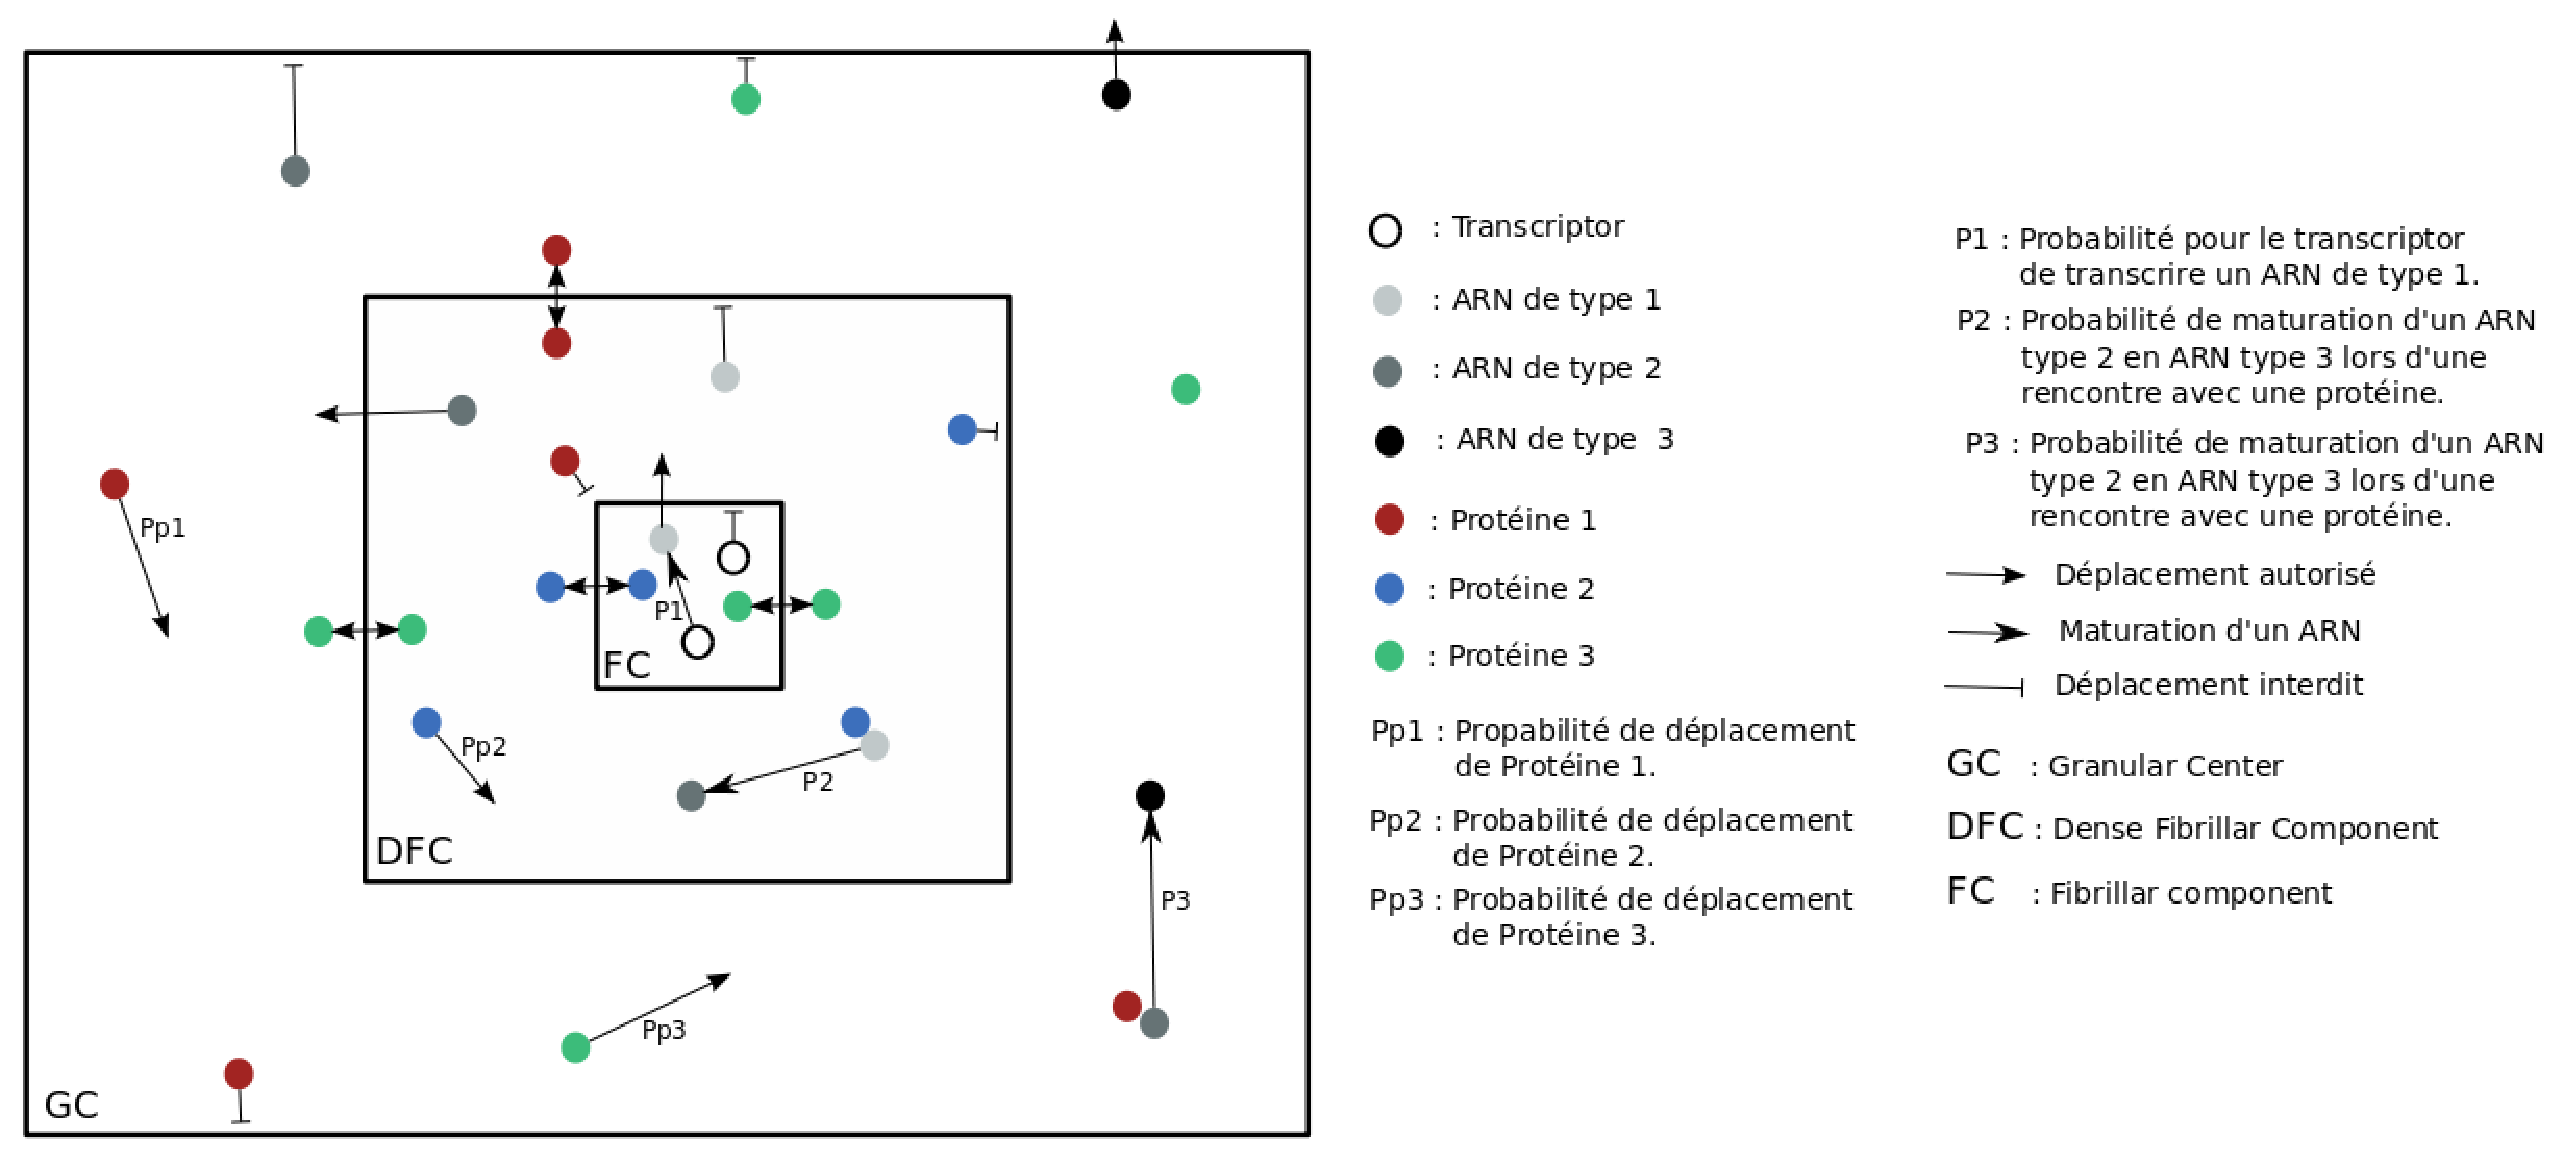
\includegraphics[width=1\columnwidth]{img/schemaSimu.pdf}
  \end{center}

\end{frame}

\subsection{Prototypage de l'interface}

\begin{frame}
  \frametitle{}

  \begin{block}{}
  \begin{center}
    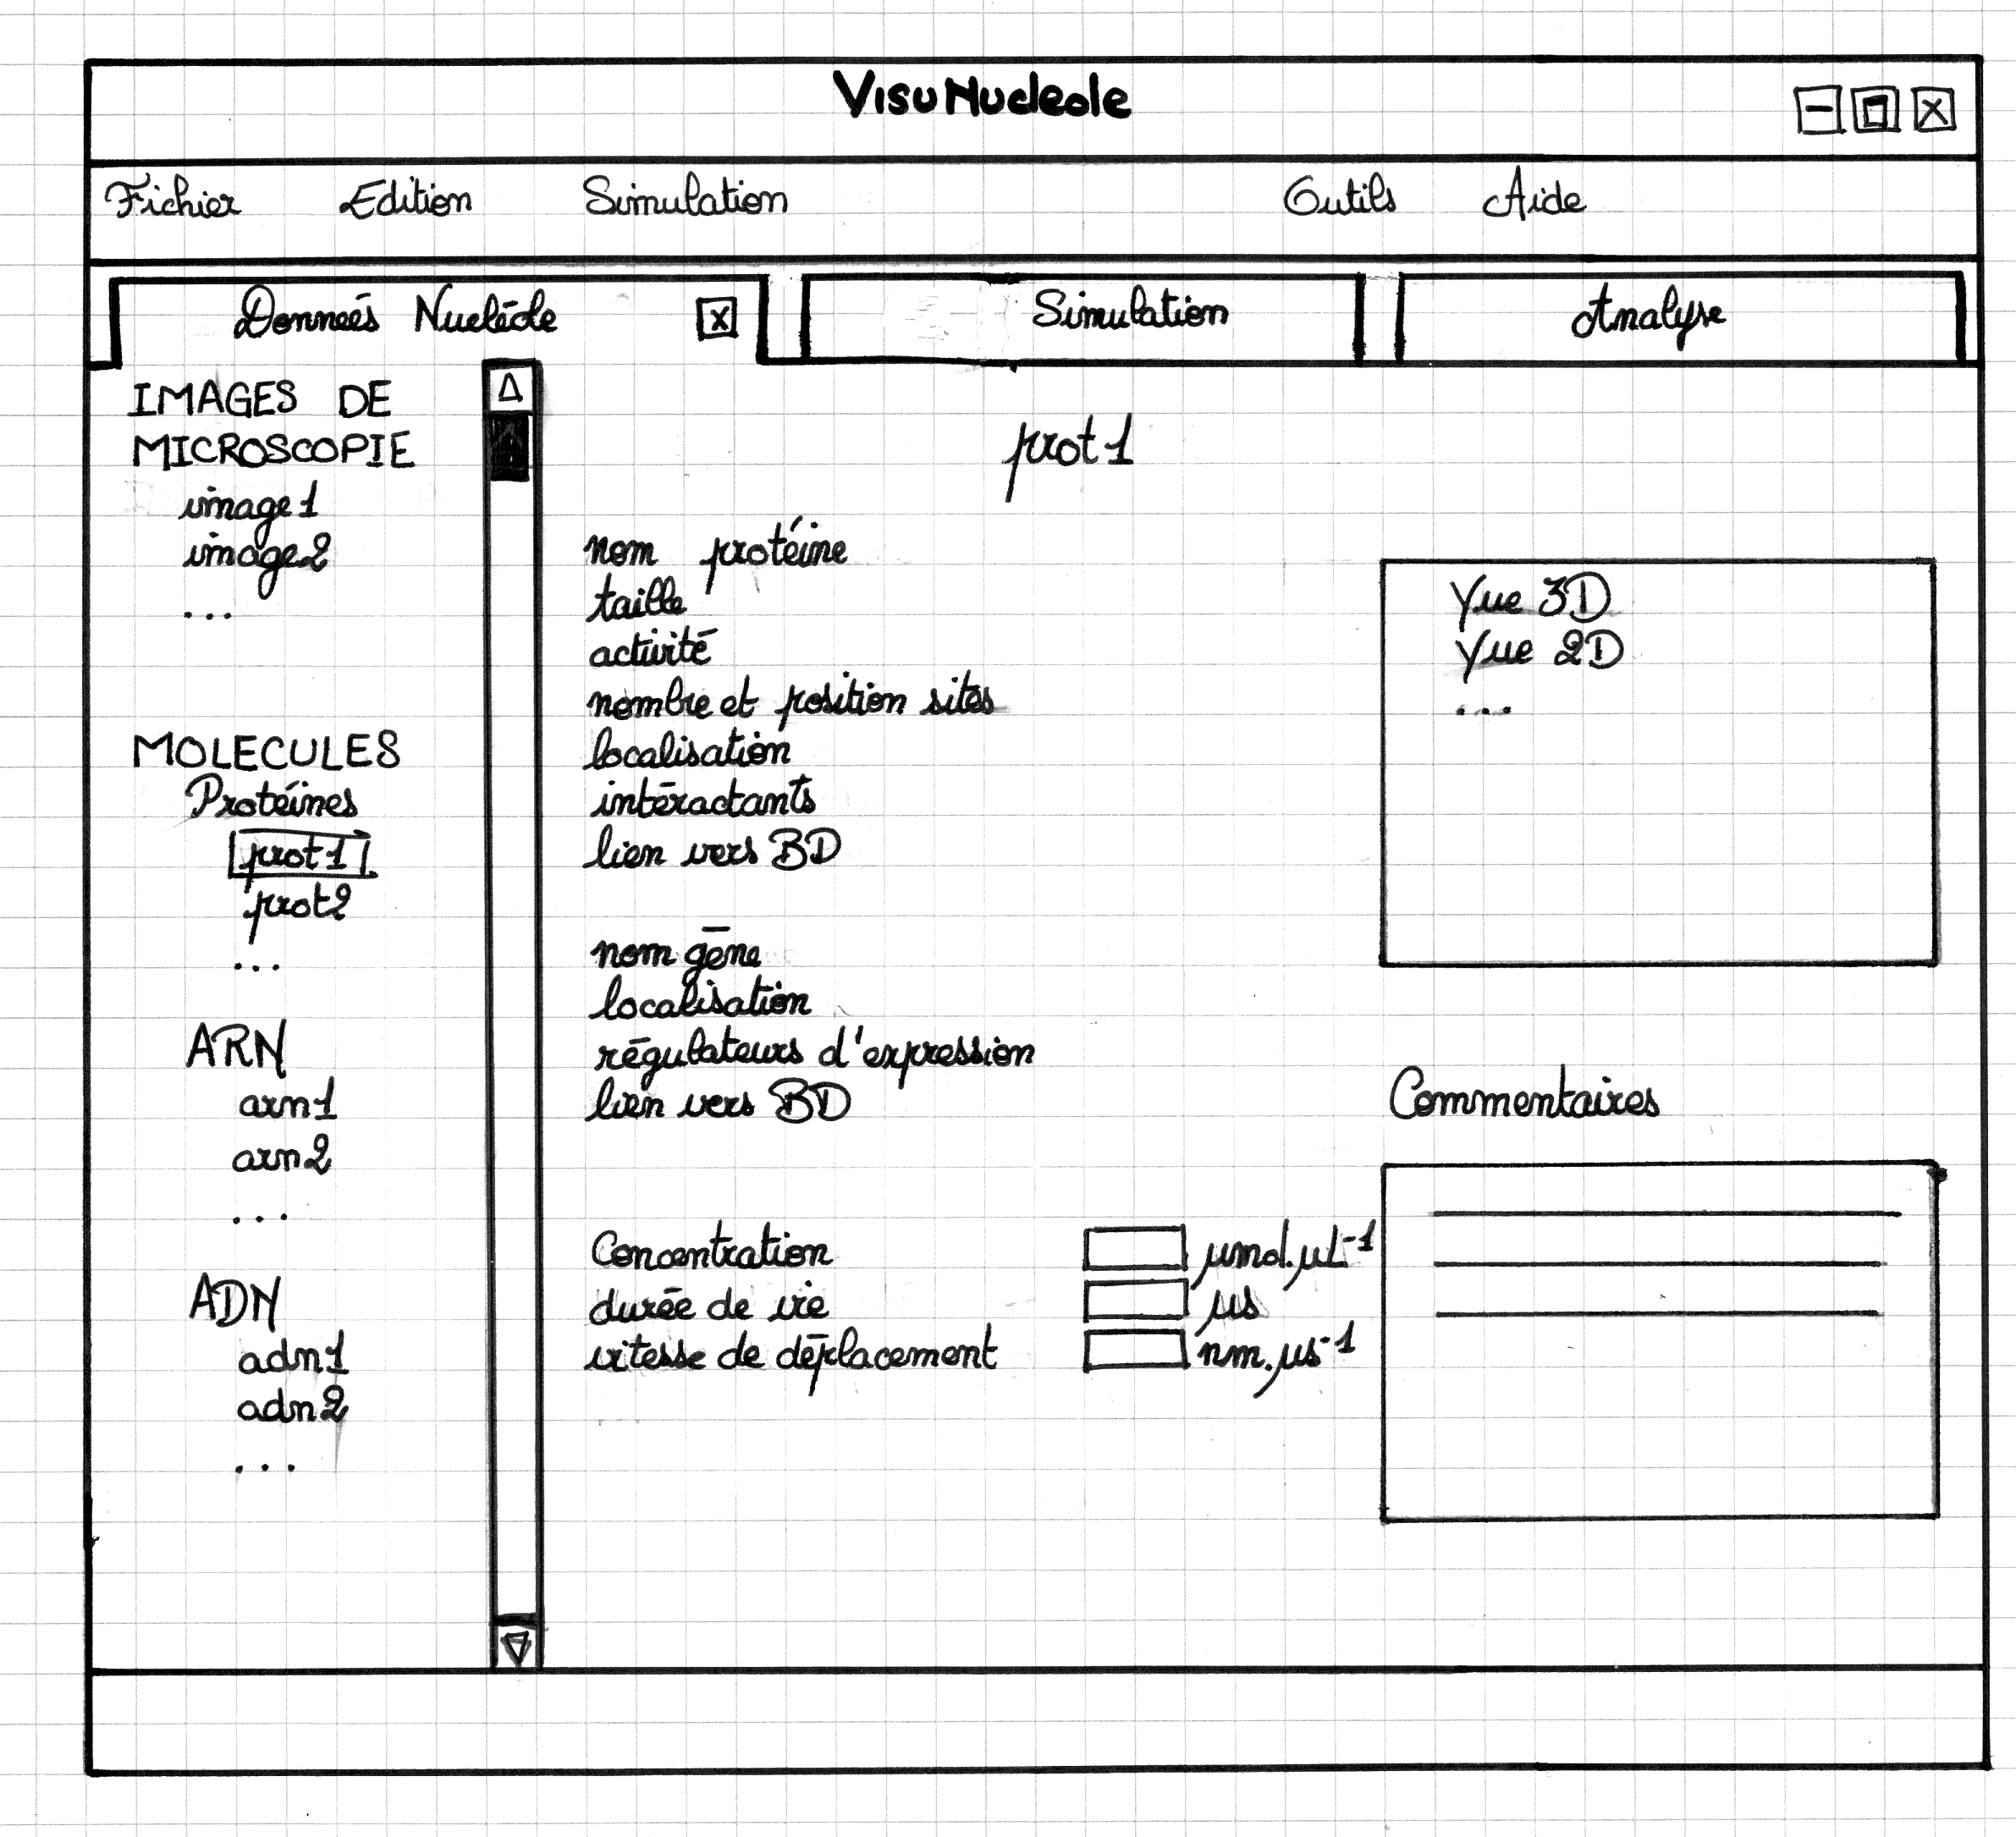
\includegraphics[width=0.7\columnwidth]{img/mock1.png}
  \end{center}
  \end{block}

\end{frame}

\section{Réalisation}

\subsection{Technologies utilisées}

\begin{frame}
  \frametitle{}

  \begin{block}{Qt / C++}
    \begin{itemize}
    \item Performance de calculs
    \item Qt en tant que framework : 
      \begin{itemize}
      \item Multiplateforme
      \item Rapidité de développement
      \end{itemize}
    \end{itemize}
  \end{block}
  
\end{frame}

\begin{frame}
  \frametitle{SGBD}

  \begin{block}{Architecture modulable}
    \begin{itemize}
    \item Possibilité d'ajouter des interfaces à des SGBD
    \item Choix du XML :
    \item Inconvénient : 
    \end{itemize}
  \end{block}

  \begin{block}{XML comme SGBD}
    \begin{itemize}
    \item Léger :  pas besoin de serveur
    \item Format répandu : nombreuses bibliothèques
    \item Inconvénient : 
    \end{itemize}
  \end{block}

\end{frame}

\subsection{Diagramme de classe}

\begin{frame}

  \begin{center}
      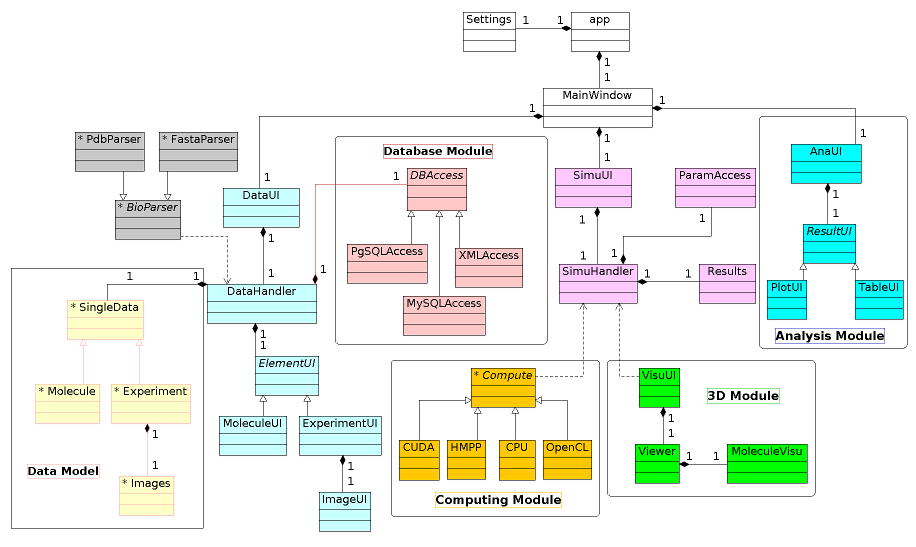
\includegraphics[width=1\columnwidth]{img/diag.png}
  \end{center}

\end{frame}

\subsection{Implémentation de la modélisation}

\begin{frame}
  \frametitle{Améliorations possibles}
  \begin{block}{}
    \begin{itemize}
    \item Calcul parallèle
    \item Calcul des densités des clusters finaux
    \item Algorithme k-médoïde
    \item Approche plus hiérarchique avec DIANA et AGNES
    \end{itemize}
  \end{block}

\end{frame}

\subsection{Réalisation de l'interface}

\begin{frame}
  \frametitle{Interface avec la base de donnée}

  \begin{center}
      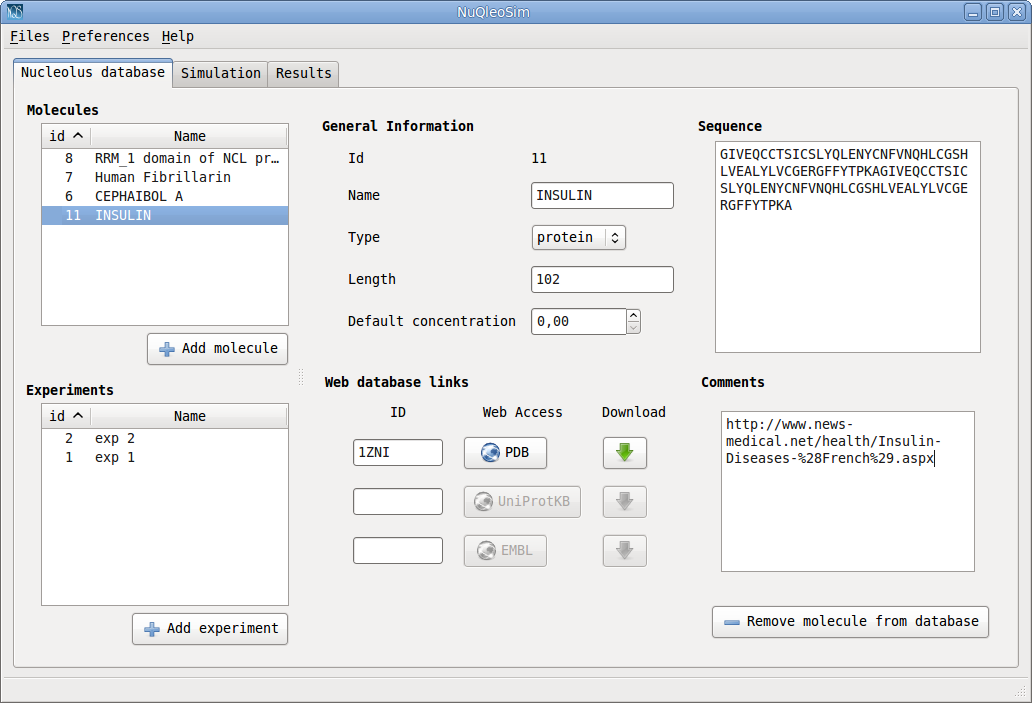
\includegraphics[width=0.9\columnwidth]{img/inter1.png}
  \end{center}

\end{frame}

\begin{frame}
  \frametitle{Paramétrage d'une simulation}

  \begin{center}
      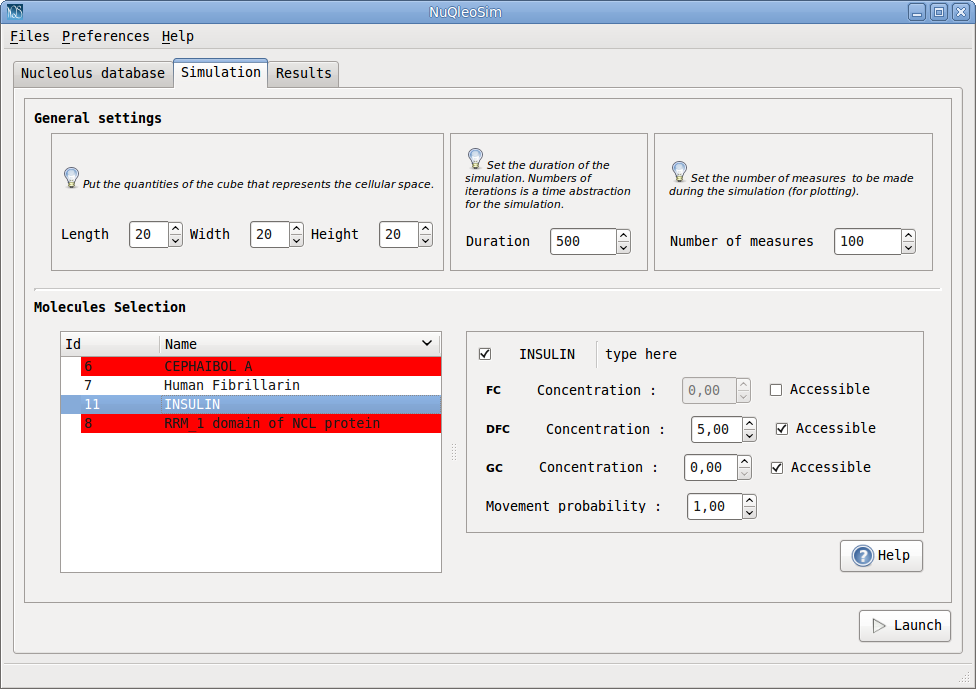
\includegraphics[width=0.9\columnwidth]{img/inter2.png}
  \end{center}

\end{frame}

\begin{frame}
  \frametitle{Visualisation de la modélisation}

    \begin{center}
      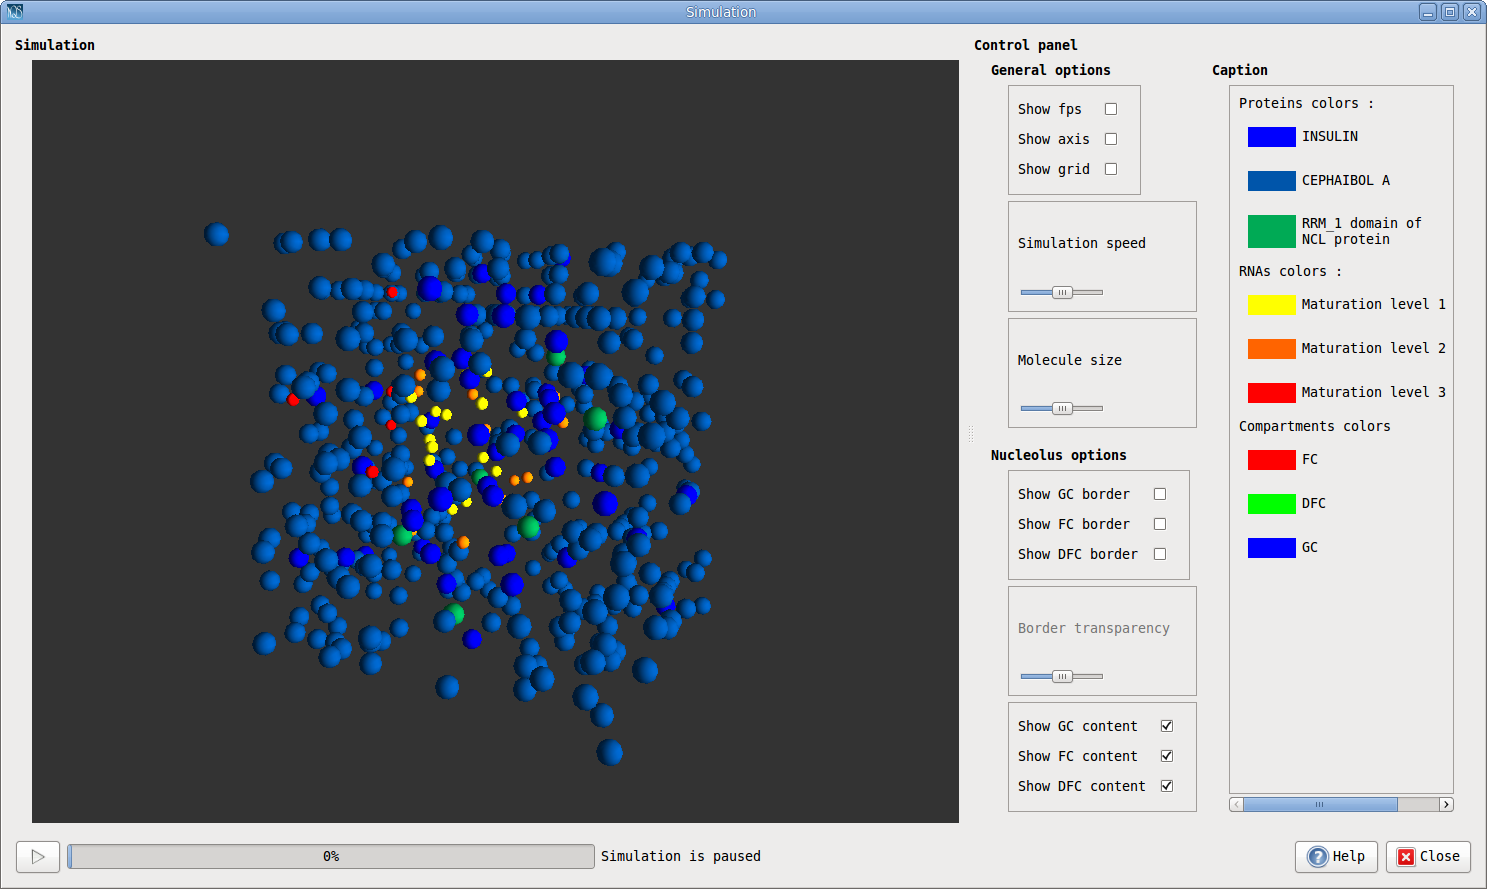
\includegraphics[width=1\columnwidth]{img/inter3.png}
  \end{center}

\end{frame}

\begin{frame}
  \frametitle{Exemple de génération de résultats}

  \begin{center}
      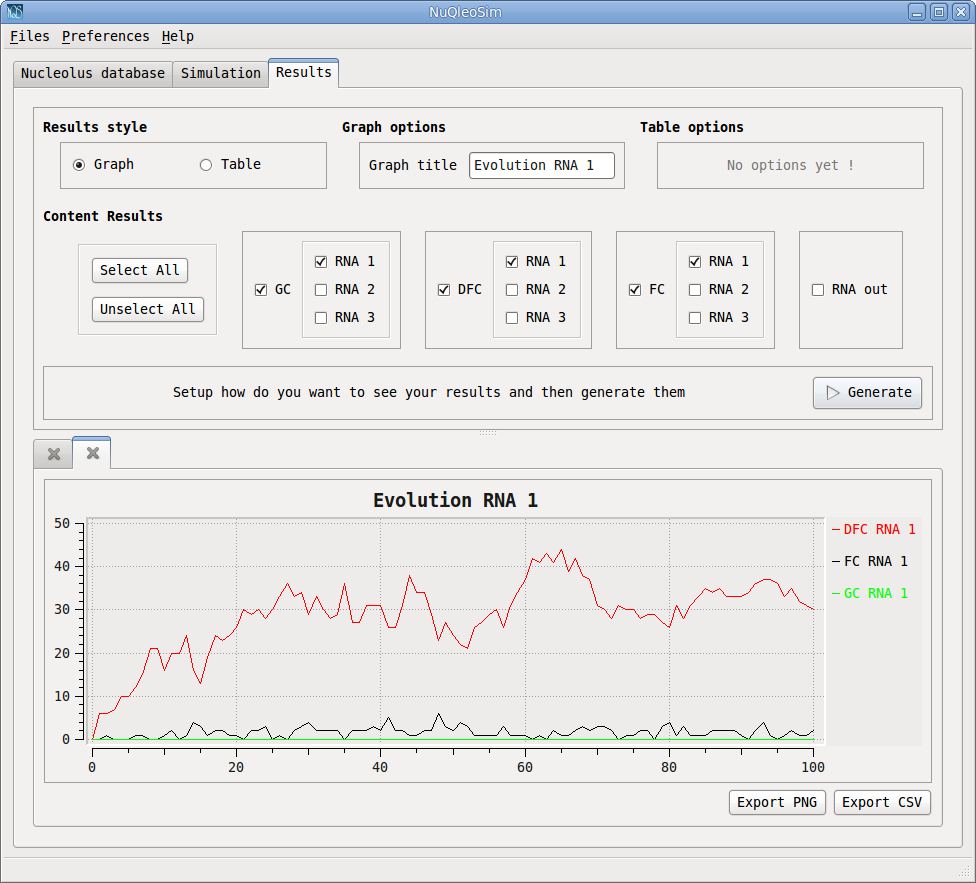
\includegraphics[width=0.7\columnwidth]{img/inter4.png}
    \end{center}

\end{frame}

\section*{Conclusion}

\begin{frame}
  \frametitle{Conclusion}

  \begin{block}{}
    \begin{itemize}
    \item Construction et exploitation d'un entrepôt de données
    \item Traitement d'un grand nombre de données
    \item Etablissement de critères en fonction d'une problématique
      biologique
    \item Outil de visualisation
    \end{itemize}
  \end{block}

\end{frame}

\begin{frame}
  \begin{center}Merci de votre attention\end{center}
\end{frame}

\end{document}

